\subsubsection{Architecture}
\label{subsubsec:architecture}
In order for our project, described in \fullref{subsec:usecase}, to succeed, it is of inestimable value to have a
architecture that supports this in the best possible way.

The requirements for our architecture are as follows:
\begin{enumerate}
  \item Multiple data sources must be supported.
  \item All data collected must be stored in its original representation to be able to answer still unknown questions at a later point in time.
  \item The areas of data acquisition, analysis and visualization must be separated.
\end{enumerate}

When dealing with large amounts of data, the following two architectural approaches distinguish between each other:

\paragraph{Lambda Architectur}
Named after the Greek $\lambda$, this approach is characterized by the fact that the streaming data is processed in two ways.
On the one hand, the data stream is routed directly to a \textit{Speed Layer}, which is often based on in-memory technology,
processes it in real time and makes it available to the \textit{Serving Layer}.
Since streams are by definition infinite and the speed layer is expensive and physically finite,
the stream is routed from \textit{Ingestion Layer} into the \textit{Batch Layer} in parallel.
This layer stores the data persistently and starts a batch job after a defined interval to process the started data and transfer it to the serving layer.
So it is the responsibility of the serving layer to mix the aggregated inventory data from the batch layer with the real-time data of the speed layer,
which has not yet been processed by the batch layer.\cite{lambda} \cite{jaxkappa}

\begin{figure}[h]
	\centering
	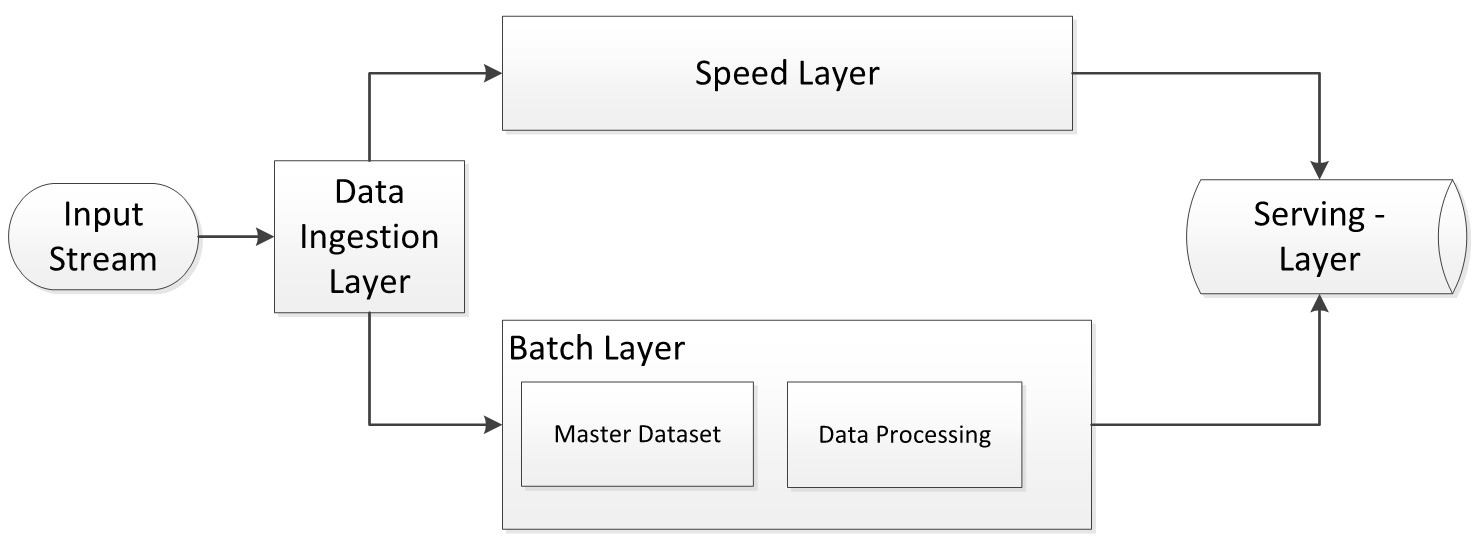
\includegraphics[width=10cm]{berle_lambda-architektur_3.jpg}
	\caption[Scheme of $\lambda$ architecture]{Scheme of $\lambda$ architecture\cite{jaxkappa}}
	\label{fig:KafkaArchitecture}
\end{figure}

\paragraph{Kappa Architectur}
This approach, designed by Confluent co-founder and CEO Jay Kreps, dispenses with batch processing and therefore only requires
\textit{Ingestion-}, \textit{Speed-} and \textit{Serving-Layer}.
This saves the development and operation of two separate layers and the time-consuming mixing of batch data with live data in the \textit{Serving-Layer}.
A prerequisite, however, is that the \textit{Ingestion-Layer} does not only pass through data volatilely,
but rather holds the raw data persistently in the \textit{Master-Dataset} as a \textit{Buffer} in order to make the raw data available again in case of a new,
not yet precalculated request or change in the \textit{Speed-Layer}.
To ensure a correct replay of the messages, the buffer is based on a canonical log, in which only messages can be added unchanged, but already saved messages can no
longer be changed or moved in their order.
This approach was named after the Greek $\kappa$ in order to illustrate both proximity and demarcation to the $\lambda$ architecture.
\cite{Kappa} \cite{Kappa2}

\begin{figure}[h]
	\centering
	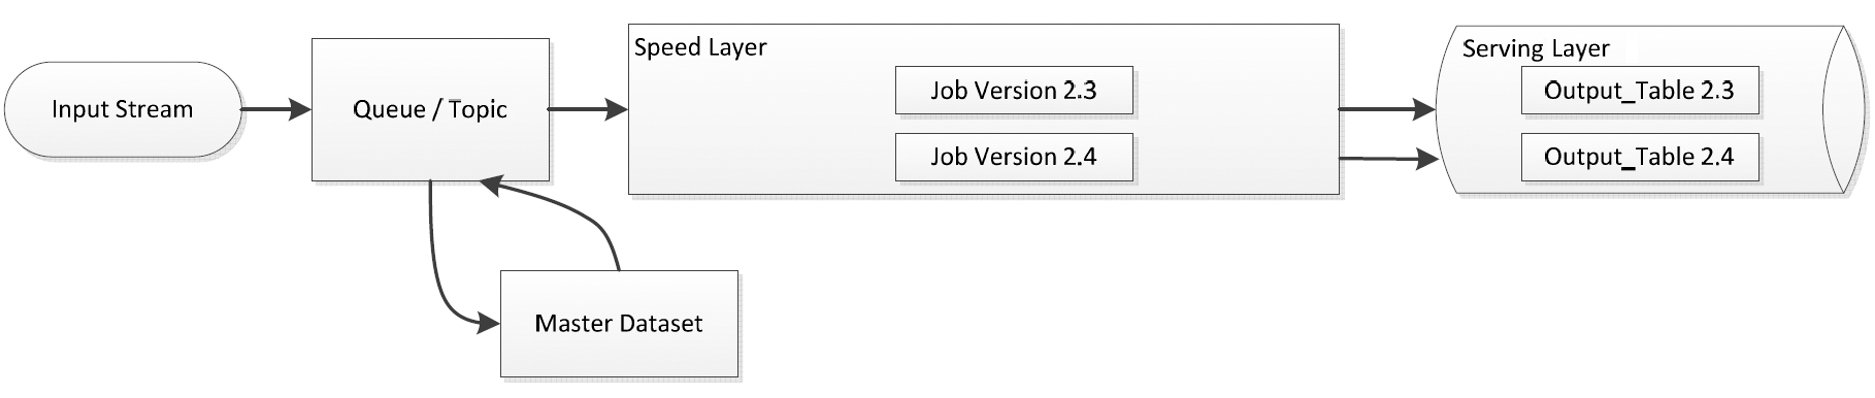
\includegraphics[width=10cm]{berle_lambda-architektur_4.jpg}
	\caption[Scheme of $\kappa$ Architectur]{Scheme of $\kappa$ Architectur\cite{jaxkappa}}
	\label{fig:KappaArchitecture}
\end{figure}

Both the Kappa and the Lamba architecture cover our requirements.
Via the input stream, any number of data sources can be accessed, in the
data ingestion layer, all collected data is stored, and then the data is processed and can be persisted in the serving layer.
The analysis part can now be executed on the serving layer.
The separation into different layers also fulfils our third requirement.

% TODO: kann das so stehen bleiben?
As explained in chapter \fullref{subsubsec:sources} our biggest data source is the Fusion \ac{API} of Yelp and
the Search \ac{API} of ImmobilienScout24.
Due to the fact that Yelp data - with the exception of the Business ID - may not be stored for more than 24 hours,\cite{YelpFaq}
the amount of data collected is manageable.

Due to the manageable amount of data that should be available to us in the end and the limited time period to complete this project,
we consciously forgo a batch layer and therefore also the Lambda architecture
in order not to unnecessarily increase the complexity of our architecture but also to reduce the processing time of data at the same time.
So we decided for a simplified version of the Kappa architecture.

In step 1, also known as \textit{Data Ingestion} we collect the data from different data sources and write them unchanged into \gds{}
The second step consists of transporting the data into the \pg{} database from where it can be analyzed later on.
The transport included not only the simple moving of the data from the source to the target database but also the conversion of the data
into a format that has been adapted to the relational database.
Conversion, in this case, does not only mean to add additional attributes to enrich the subsequent analysis and visualization in a more meaningful way,
but also sorting out not used attributes. This second step is also referred to as \textit{Data Storage}.
The last step, the analysis of the data, was done depending on the scenario either with the Bi- and Software Analysis Software Tableau\footnote{\url{https://www.tableau.com/}} or various Scripts written in either \code{Python} or \code{R}.
\newline
The following picture shows the previously described variant of the Kappa architecture.

%TODO: picture
